% Created by tikzDevice version 0.12.6 on 2025-04-17 10:37:52
% !TEX encoding = UTF-8 Unicode
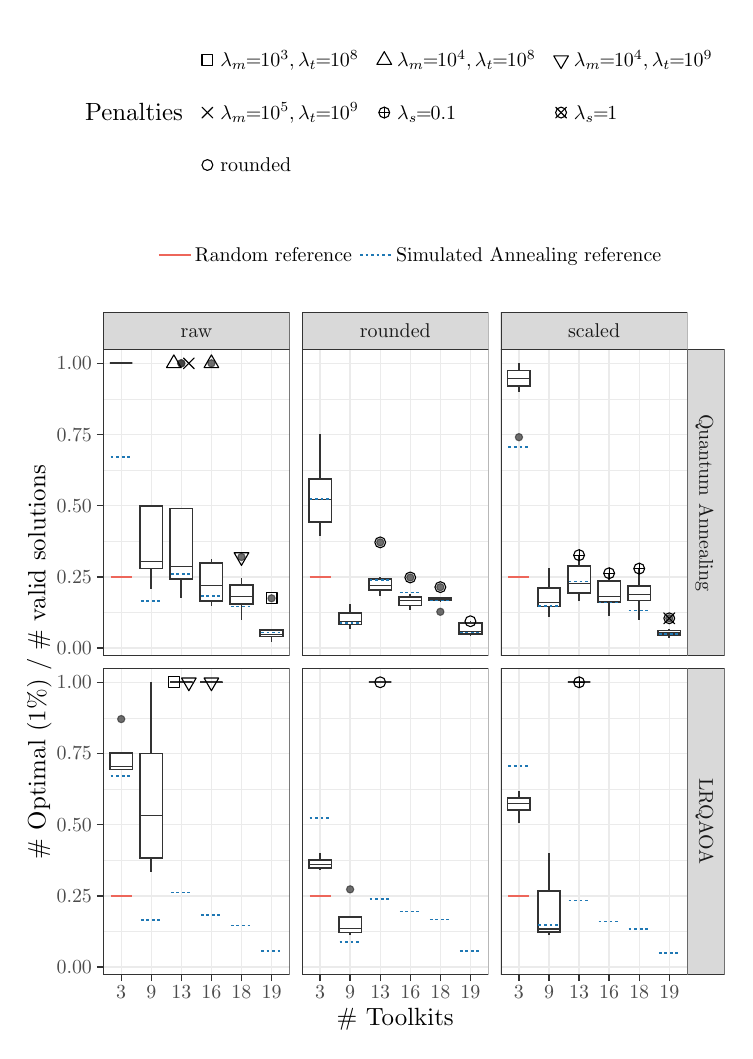
\begin{tikzpicture}[x=1pt,y=1pt]
\definecolor{fillColor}{RGB}{255,255,255}
\path[use as bounding box,fill=fillColor,fill opacity=0.00] (0,0) rectangle (251.81,362.60);
\begin{scope}
\path[clip] (  0.00,  0.00) rectangle (251.81,362.60);
\definecolor{drawColor}{RGB}{255,255,255}
\definecolor{fillColor}{RGB}{255,255,255}

\path[draw=drawColor,line width= 0.5pt,line join=round,line cap=round,fill=fillColor] (  0.00,  0.00) rectangle (251.81,362.60);
\end{scope}
\begin{scope}
\path[clip] ( 27.28,135.60) rectangle ( 94.64,246.34);
\definecolor{fillColor}{RGB}{255,255,255}

\path[fill=fillColor] ( 27.28,135.60) rectangle ( 94.64,246.34);
\definecolor{drawColor}{gray}{0.92}

\path[draw=drawColor,line width= 0.2pt,line join=round] ( 27.28,151.27) --
	( 94.64,151.27);

\path[draw=drawColor,line width= 0.2pt,line join=round] ( 27.28,177.00) --
	( 94.64,177.00);

\path[draw=drawColor,line width= 0.2pt,line join=round] ( 27.28,202.72) --
	( 94.64,202.72);

\path[draw=drawColor,line width= 0.2pt,line join=round] ( 27.28,228.44) --
	( 94.64,228.44);

\path[draw=drawColor,line width= 0.5pt,line join=round] ( 27.28,138.41) --
	( 94.64,138.41);

\path[draw=drawColor,line width= 0.5pt,line join=round] ( 27.28,164.13) --
	( 94.64,164.13);

\path[draw=drawColor,line width= 0.5pt,line join=round] ( 27.28,189.86) --
	( 94.64,189.86);

\path[draw=drawColor,line width= 0.5pt,line join=round] ( 27.28,215.58) --
	( 94.64,215.58);

\path[draw=drawColor,line width= 0.5pt,line join=round] ( 27.28,241.31) --
	( 94.64,241.31);

\path[draw=drawColor,line width= 0.5pt,line join=round] ( 33.80,135.60) --
	( 33.80,246.34);

\path[draw=drawColor,line width= 0.5pt,line join=round] ( 44.66,135.60) --
	( 44.66,246.34);

\path[draw=drawColor,line width= 0.5pt,line join=round] ( 55.52,135.60) --
	( 55.52,246.34);

\path[draw=drawColor,line width= 0.5pt,line join=round] ( 66.39,135.60) --
	( 66.39,246.34);

\path[draw=drawColor,line width= 0.5pt,line join=round] ( 77.25,135.60) --
	( 77.25,246.34);

\path[draw=drawColor,line width= 0.5pt,line join=round] ( 88.12,135.60) --
	( 88.12,246.34);
\definecolor{drawColor}{gray}{0.20}

\path[draw=drawColor,line width= 0.6pt,line join=round] ( 33.80,241.31) -- ( 33.80,241.31);

\path[draw=drawColor,line width= 0.6pt,line join=round] ( 33.80,241.31) -- ( 33.80,241.31);

\path[draw=drawColor,line width= 0.6pt,fill=fillColor] ( 29.72,241.31) --
	( 29.72,241.31) --
	( 37.87,241.31) --
	( 37.87,241.31) --
	( 29.72,241.31) --
	cycle;

\path[draw=drawColor,line width= 0.4pt] ( 29.72,241.31) -- ( 37.87,241.31);

\path[draw=drawColor,line width= 0.6pt,line join=round] ( 44.66,189.86) -- ( 44.66,189.86);

\path[draw=drawColor,line width= 0.6pt,line join=round] ( 44.66,167.14) -- ( 44.66,159.66);

\path[draw=drawColor,line width= 0.6pt,fill=fillColor] ( 40.59,189.86) --
	( 40.59,167.14) --
	( 48.73,167.14) --
	( 48.73,189.86) --
	( 40.59,189.86) --
	cycle;

\path[draw=drawColor,line width= 0.4pt] ( 40.59,169.79) -- ( 48.73,169.79);
\definecolor{drawColor}{RGB}{51,51,51}
\definecolor{fillColor}{RGB}{51,51,51}

\path[draw=drawColor,draw opacity=0.70,line width= 0.4pt,line join=round,line cap=round,fill=fillColor,fill opacity=0.70] ( 55.52,241.31) circle (  1.31);

\path[draw=drawColor,draw opacity=0.70,line width= 0.4pt,line join=round,line cap=round,fill=fillColor,fill opacity=0.70] ( 55.52,241.31) circle (  1.31);
\definecolor{drawColor}{gray}{0.20}

\path[draw=drawColor,line width= 0.6pt,line join=round] ( 55.52,188.89) -- ( 55.52,188.89);

\path[draw=drawColor,line width= 0.6pt,line join=round] ( 55.52,163.49) -- ( 55.52,156.35);
\definecolor{fillColor}{RGB}{255,255,255}

\path[draw=drawColor,line width= 0.6pt,fill=fillColor] ( 51.45,188.89) --
	( 51.45,163.49) --
	( 59.60,163.49) --
	( 59.60,188.89) --
	( 51.45,188.89) --
	cycle;

\path[draw=drawColor,line width= 0.4pt] ( 51.45,167.81) -- ( 59.60,167.81);
\definecolor{drawColor}{RGB}{51,51,51}
\definecolor{fillColor}{RGB}{51,51,51}

\path[draw=drawColor,draw opacity=0.70,line width= 0.4pt,line join=round,line cap=round,fill=fillColor,fill opacity=0.70] ( 66.39,241.31) circle (  1.31);
\definecolor{drawColor}{gray}{0.20}

\path[draw=drawColor,line width= 0.6pt,line join=round] ( 66.39,169.11) -- ( 66.39,170.52);

\path[draw=drawColor,line width= 0.6pt,line join=round] ( 66.39,155.32) -- ( 66.39,153.47);
\definecolor{fillColor}{RGB}{255,255,255}

\path[draw=drawColor,line width= 0.6pt,fill=fillColor] ( 62.32,169.11) --
	( 62.32,155.32) --
	( 70.46,155.32) --
	( 70.46,169.11) --
	( 62.32,169.11) --
	cycle;

\path[draw=drawColor,line width= 0.4pt] ( 62.32,161.17) -- ( 70.46,161.17);
\definecolor{drawColor}{RGB}{51,51,51}
\definecolor{fillColor}{RGB}{51,51,51}

\path[draw=drawColor,draw opacity=0.70,line width= 0.4pt,line join=round,line cap=round,fill=fillColor,fill opacity=0.70] ( 77.25,171.34) circle (  1.31);
\definecolor{drawColor}{gray}{0.20}

\path[draw=drawColor,line width= 0.6pt,line join=round] ( 77.25,161.16) -- ( 77.25,163.80);

\path[draw=drawColor,line width= 0.6pt,line join=round] ( 77.25,154.44) -- ( 77.25,148.52);
\definecolor{fillColor}{RGB}{255,255,255}

\path[draw=drawColor,line width= 0.6pt,fill=fillColor] ( 73.18,161.16) --
	( 73.18,154.44) --
	( 81.33,154.44) --
	( 81.33,161.16) --
	( 73.18,161.16) --
	cycle;

\path[draw=drawColor,line width= 0.4pt] ( 73.18,156.90) -- ( 81.33,156.90);
\definecolor{drawColor}{RGB}{51,51,51}
\definecolor{fillColor}{RGB}{51,51,51}

\path[draw=drawColor,draw opacity=0.70,line width= 0.4pt,line join=round,line cap=round,fill=fillColor,fill opacity=0.70] ( 88.12,156.40) circle (  1.31);
\definecolor{drawColor}{gray}{0.20}

\path[draw=drawColor,line width= 0.6pt,line join=round] ( 88.12,144.94) -- ( 88.12,145.24);

\path[draw=drawColor,line width= 0.6pt,line join=round] ( 88.12,142.62) -- ( 88.12,140.63);
\definecolor{fillColor}{RGB}{255,255,255}

\path[draw=drawColor,line width= 0.6pt,fill=fillColor] ( 84.04,144.94) --
	( 84.04,142.62) --
	( 92.19,142.62) --
	( 92.19,144.94) --
	( 84.04,144.94) --
	cycle;

\path[draw=drawColor,line width= 0.4pt] ( 84.04,143.48) -- ( 92.19,143.48);
\definecolor{drawColor}{RGB}{0,0,0}

\path[draw=drawColor,line width= 0.4pt,line join=round,line cap=round] ( 66.39,244.36) --
	( 69.03,239.78) --
	( 63.75,239.78) --
	cycle;

\path[draw=drawColor,line width= 0.4pt,line join=round,line cap=round] ( 86.16,154.44) rectangle ( 90.08,158.36);

\path[draw=drawColor,line width= 0.4pt,line join=round,line cap=round] ( 56.28,239.34) -- ( 60.20,243.27);

\path[draw=drawColor,line width= 0.4pt,line join=round,line cap=round] ( 56.28,243.27) -- ( 60.20,239.34);

\path[draw=drawColor,line width= 0.4pt,line join=round,line cap=round] ( 52.81,244.36) --
	( 55.45,239.78) --
	( 50.17,239.78) --
	cycle;

\path[draw=drawColor,line width= 0.4pt,line join=round,line cap=round] ( 77.25,168.29) --
	( 79.90,172.86) --
	( 74.61,172.86) --
	cycle;
\definecolor{drawColor}{RGB}{237,102,90}

\path[draw=drawColor,line width= 0.6pt,line join=round] ( 29.99,164.13) -- ( 37.60,164.13);
\definecolor{drawColor}{RGB}{31,120,180}

\path[draw=drawColor,line width= 0.6pt,dash pattern=on 1pt off 1pt ,line join=round] ( 40.86,155.47) -- ( 48.46,155.47);

\path[draw=drawColor,line width= 0.6pt,dash pattern=on 1pt off 1pt ,line join=round] ( 73.45,153.38) -- ( 81.06,153.38);

\path[draw=drawColor,line width= 0.6pt,dash pattern=on 1pt off 1pt ,line join=round] ( 51.72,165.28) -- ( 59.33,165.28);

\path[draw=drawColor,line width= 0.6pt,dash pattern=on 1pt off 1pt ,line join=round] ( 62.59,157.14) -- ( 70.19,157.14);

\path[draw=drawColor,line width= 0.6pt,dash pattern=on 1pt off 1pt ,line join=round] ( 29.99,207.46) -- ( 37.60,207.46);

\path[draw=drawColor,line width= 0.6pt,dash pattern=on 1pt off 1pt ,line join=round] ( 84.32,144.10) -- ( 91.92,144.10);
\definecolor{drawColor}{gray}{0.20}

\path[draw=drawColor,line width= 0.5pt,line join=round,line cap=round] ( 27.28,135.60) rectangle ( 94.64,246.34);
\end{scope}
\begin{scope}
\path[clip] ( 27.28, 20.35) rectangle ( 94.64,131.10);
\definecolor{fillColor}{RGB}{255,255,255}

\path[fill=fillColor] ( 27.28, 20.35) rectangle ( 94.64,131.10);
\definecolor{drawColor}{gray}{0.92}

\path[draw=drawColor,line width= 0.2pt,line join=round] ( 27.28, 36.03) --
	( 94.64, 36.03);

\path[draw=drawColor,line width= 0.2pt,line join=round] ( 27.28, 61.75) --
	( 94.64, 61.75);

\path[draw=drawColor,line width= 0.2pt,line join=round] ( 27.28, 87.48) --
	( 94.64, 87.48);

\path[draw=drawColor,line width= 0.2pt,line join=round] ( 27.28,113.20) --
	( 94.64,113.20);

\path[draw=drawColor,line width= 0.5pt,line join=round] ( 27.28, 23.17) --
	( 94.64, 23.17);

\path[draw=drawColor,line width= 0.5pt,line join=round] ( 27.28, 48.89) --
	( 94.64, 48.89);

\path[draw=drawColor,line width= 0.5pt,line join=round] ( 27.28, 74.61) --
	( 94.64, 74.61);

\path[draw=drawColor,line width= 0.5pt,line join=round] ( 27.28,100.34) --
	( 94.64,100.34);

\path[draw=drawColor,line width= 0.5pt,line join=round] ( 27.28,126.06) --
	( 94.64,126.06);

\path[draw=drawColor,line width= 0.5pt,line join=round] ( 33.80, 20.35) --
	( 33.80,131.10);

\path[draw=drawColor,line width= 0.5pt,line join=round] ( 44.66, 20.35) --
	( 44.66,131.10);

\path[draw=drawColor,line width= 0.5pt,line join=round] ( 55.52, 20.35) --
	( 55.52,131.10);

\path[draw=drawColor,line width= 0.5pt,line join=round] ( 66.39, 20.35) --
	( 66.39,131.10);

\path[draw=drawColor,line width= 0.5pt,line join=round] ( 77.25, 20.35) --
	( 77.25,131.10);

\path[draw=drawColor,line width= 0.5pt,line join=round] ( 88.12, 20.35) --
	( 88.12,131.10);
\definecolor{drawColor}{RGB}{51,51,51}
\definecolor{fillColor}{RGB}{51,51,51}

\path[draw=drawColor,draw opacity=0.70,line width= 0.4pt,line join=round,line cap=round,fill=fillColor,fill opacity=0.70] ( 33.80,112.76) circle (  1.31);
\definecolor{drawColor}{gray}{0.20}

\path[draw=drawColor,line width= 0.6pt,line join=round] ( 33.80,100.48) -- ( 33.80,100.48);

\path[draw=drawColor,line width= 0.6pt,line join=round] ( 33.80, 94.56) -- ( 33.80, 94.49);
\definecolor{fillColor}{RGB}{255,255,255}

\path[draw=drawColor,line width= 0.6pt,fill=fillColor] ( 29.72,100.48) --
	( 29.72, 94.56) --
	( 37.87, 94.56) --
	( 37.87,100.48) --
	( 29.72,100.48) --
	cycle;

\path[draw=drawColor,line width= 0.4pt] ( 29.72, 95.48) -- ( 37.87, 95.48);

\path[draw=drawColor,line width= 0.6pt,line join=round] ( 44.66,100.34) -- ( 44.66,126.06);

\path[draw=drawColor,line width= 0.6pt,line join=round] ( 44.66, 62.61) -- ( 44.66, 57.46);

\path[draw=drawColor,line width= 0.6pt,fill=fillColor] ( 40.59,100.34) --
	( 40.59, 62.61) --
	( 48.73, 62.61) --
	( 48.73,100.34) --
	( 40.59,100.34) --
	cycle;

\path[draw=drawColor,line width= 0.4pt] ( 40.59, 78.04) -- ( 48.73, 78.04);

\path[draw=drawColor,line width= 0.6pt,line join=round] ( 55.52,126.06) -- ( 55.52,126.06);

\path[draw=drawColor,line width= 0.6pt,line join=round] ( 55.52,126.06) -- ( 55.52,126.06);

\path[draw=drawColor,line width= 0.6pt,fill=fillColor] ( 51.45,126.06) --
	( 51.45,126.06) --
	( 59.60,126.06) --
	( 59.60,126.06) --
	( 51.45,126.06) --
	cycle;

\path[draw=drawColor,line width= 0.4pt] ( 51.45,126.06) -- ( 59.60,126.06);

\path[draw=drawColor,line width= 0.6pt,line join=round] ( 66.39,126.06) -- ( 66.39,126.06);

\path[draw=drawColor,line width= 0.6pt,line join=round] ( 66.39,126.06) -- ( 66.39,126.06);

\path[draw=drawColor,line width= 0.6pt,fill=fillColor] ( 62.32,126.06) --
	( 62.32,126.06) --
	( 70.46,126.06) --
	( 70.46,126.06) --
	( 62.32,126.06) --
	cycle;

\path[draw=drawColor,line width= 0.4pt] ( 62.32,126.06) -- ( 70.46,126.06);
\definecolor{drawColor}{RGB}{0,0,0}

\path[draw=drawColor,line width= 0.4pt,line join=round,line cap=round] ( 58.24,123.01) --
	( 60.88,127.59) --
	( 55.60,127.59) --
	cycle;

\path[draw=drawColor,line width= 0.4pt,line join=round,line cap=round] ( 50.85,124.10) rectangle ( 54.77,128.02);

\path[draw=drawColor,line width= 0.4pt,line join=round,line cap=round] ( 66.39,123.01) --
	( 69.03,127.59) --
	( 63.75,127.59) --
	cycle;
\definecolor{drawColor}{RGB}{237,102,90}

\path[draw=drawColor,line width= 0.6pt,line join=round] ( 29.99, 48.89) -- ( 37.60, 48.89);
\definecolor{drawColor}{RGB}{31,120,180}

\path[draw=drawColor,line width= 0.6pt,dash pattern=on 1pt off 1pt ,line join=round] ( 40.86, 40.22) -- ( 48.46, 40.22);

\path[draw=drawColor,line width= 0.6pt,dash pattern=on 1pt off 1pt ,line join=round] ( 73.45, 38.13) -- ( 81.06, 38.13);

\path[draw=drawColor,line width= 0.6pt,dash pattern=on 1pt off 1pt ,line join=round] ( 51.72, 50.04) -- ( 59.33, 50.04);

\path[draw=drawColor,line width= 0.6pt,dash pattern=on 1pt off 1pt ,line join=round] ( 62.59, 41.89) -- ( 70.19, 41.89);

\path[draw=drawColor,line width= 0.6pt,dash pattern=on 1pt off 1pt ,line join=round] ( 29.99, 92.22) -- ( 37.60, 92.22);

\path[draw=drawColor,line width= 0.6pt,dash pattern=on 1pt off 1pt ,line join=round] ( 84.32, 28.86) -- ( 91.92, 28.86);
\definecolor{drawColor}{gray}{0.20}

\path[draw=drawColor,line width= 0.5pt,line join=round,line cap=round] ( 27.28, 20.35) rectangle ( 94.64,131.10);
\end{scope}
\begin{scope}
\path[clip] ( 99.14,135.60) rectangle (166.50,246.34);
\definecolor{fillColor}{RGB}{255,255,255}

\path[fill=fillColor] ( 99.14,135.60) rectangle (166.50,246.34);
\definecolor{drawColor}{gray}{0.92}

\path[draw=drawColor,line width= 0.2pt,line join=round] ( 99.14,151.27) --
	(166.50,151.27);

\path[draw=drawColor,line width= 0.2pt,line join=round] ( 99.14,177.00) --
	(166.50,177.00);

\path[draw=drawColor,line width= 0.2pt,line join=round] ( 99.14,202.72) --
	(166.50,202.72);

\path[draw=drawColor,line width= 0.2pt,line join=round] ( 99.14,228.44) --
	(166.50,228.44);

\path[draw=drawColor,line width= 0.5pt,line join=round] ( 99.14,138.41) --
	(166.50,138.41);

\path[draw=drawColor,line width= 0.5pt,line join=round] ( 99.14,164.13) --
	(166.50,164.13);

\path[draw=drawColor,line width= 0.5pt,line join=round] ( 99.14,189.86) --
	(166.50,189.86);

\path[draw=drawColor,line width= 0.5pt,line join=round] ( 99.14,215.58) --
	(166.50,215.58);

\path[draw=drawColor,line width= 0.5pt,line join=round] ( 99.14,241.31) --
	(166.50,241.31);

\path[draw=drawColor,line width= 0.5pt,line join=round] (105.66,135.60) --
	(105.66,246.34);

\path[draw=drawColor,line width= 0.5pt,line join=round] (116.52,135.60) --
	(116.52,246.34);

\path[draw=drawColor,line width= 0.5pt,line join=round] (127.39,135.60) --
	(127.39,246.34);

\path[draw=drawColor,line width= 0.5pt,line join=round] (138.25,135.60) --
	(138.25,246.34);

\path[draw=drawColor,line width= 0.5pt,line join=round] (149.12,135.60) --
	(149.12,246.34);

\path[draw=drawColor,line width= 0.5pt,line join=round] (159.98,135.60) --
	(159.98,246.34);
\definecolor{drawColor}{gray}{0.20}

\path[draw=drawColor,line width= 0.6pt,line join=round] (105.66,199.59) -- (105.66,215.73);

\path[draw=drawColor,line width= 0.6pt,line join=round] (105.66,183.99) -- (105.66,179.02);

\path[draw=drawColor,line width= 0.6pt,fill=fillColor] (101.58,199.59) --
	(101.58,183.99) --
	(109.73,183.99) --
	(109.73,199.59) --
	(101.58,199.59) --
	cycle;

\path[draw=drawColor,line width= 0.4pt] (101.58,192.20) -- (109.73,192.20);

\path[draw=drawColor,line width= 0.6pt,line join=round] (116.52,151.17) -- (116.52,154.45);

\path[draw=drawColor,line width= 0.6pt,line join=round] (116.52,146.90) -- (116.52,145.23);

\path[draw=drawColor,line width= 0.6pt,fill=fillColor] (112.45,151.17) --
	(112.45,146.90) --
	(120.60,146.90) --
	(120.60,151.17) --
	(112.45,151.17) --
	cycle;

\path[draw=drawColor,line width= 0.4pt] (112.45,148.02) -- (120.60,148.02);
\definecolor{drawColor}{RGB}{51,51,51}
\definecolor{fillColor}{RGB}{51,51,51}

\path[draw=drawColor,draw opacity=0.70,line width= 0.4pt,line join=round,line cap=round,fill=fillColor,fill opacity=0.70] (127.39,176.61) circle (  1.31);
\definecolor{drawColor}{gray}{0.20}

\path[draw=drawColor,line width= 0.6pt,line join=round] (127.39,163.48) -- (127.39,164.21);

\path[draw=drawColor,line width= 0.6pt,line join=round] (127.39,159.34) -- (127.39,157.37);
\definecolor{fillColor}{RGB}{255,255,255}

\path[draw=drawColor,line width= 0.6pt,fill=fillColor] (123.31,163.48) --
	(123.31,159.34) --
	(131.46,159.34) --
	(131.46,163.48) --
	(123.31,163.48) --
	cycle;

\path[draw=drawColor,line width= 0.4pt] (123.31,161.12) -- (131.46,161.12);
\definecolor{drawColor}{RGB}{51,51,51}
\definecolor{fillColor}{RGB}{51,51,51}

\path[draw=drawColor,draw opacity=0.70,line width= 0.4pt,line join=round,line cap=round,fill=fillColor,fill opacity=0.70] (138.25,163.93) circle (  1.31);
\definecolor{drawColor}{gray}{0.20}

\path[draw=drawColor,line width= 0.6pt,line join=round] (138.25,156.96) -- (138.25,158.00);

\path[draw=drawColor,line width= 0.6pt,line join=round] (138.25,153.76) -- (138.25,152.22);
\definecolor{fillColor}{RGB}{255,255,255}

\path[draw=drawColor,line width= 0.6pt,fill=fillColor] (134.18,156.96) --
	(134.18,153.76) --
	(142.33,153.76) --
	(142.33,156.96) --
	(134.18,156.96) --
	cycle;

\path[draw=drawColor,line width= 0.4pt] (134.18,155.68) -- (142.33,155.68);
\definecolor{drawColor}{RGB}{51,51,51}
\definecolor{fillColor}{RGB}{51,51,51}

\path[draw=drawColor,draw opacity=0.70,line width= 0.4pt,line join=round,line cap=round,fill=fillColor,fill opacity=0.70] (149.12,151.53) circle (  1.31);

\path[draw=drawColor,draw opacity=0.70,line width= 0.4pt,line join=round,line cap=round,fill=fillColor,fill opacity=0.70] (149.12,160.44) circle (  1.31);
\definecolor{drawColor}{gray}{0.20}

\path[draw=drawColor,line width= 0.6pt,line join=round] (149.12,156.51) -- (149.12,156.90);

\path[draw=drawColor,line width= 0.6pt,line join=round] (149.12,155.56) -- (149.12,155.43);
\definecolor{fillColor}{RGB}{255,255,255}

\path[draw=drawColor,line width= 0.6pt,fill=fillColor] (145.04,156.51) --
	(145.04,155.56) --
	(153.19,155.56) --
	(153.19,156.51) --
	(145.04,156.51) --
	cycle;

\path[draw=drawColor,line width= 0.4pt] (145.04,156.08) -- (153.19,156.08);

\path[draw=drawColor,line width= 0.6pt,line join=round] (159.98,147.44) -- (159.98,148.11);

\path[draw=drawColor,line width= 0.6pt,line join=round] (159.98,143.53) -- (159.98,142.75);

\path[draw=drawColor,line width= 0.6pt,fill=fillColor] (155.91,147.44) --
	(155.91,143.53) --
	(164.05,143.53) --
	(164.05,147.44) --
	(155.91,147.44) --
	cycle;

\path[draw=drawColor,line width= 0.4pt] (155.91,144.35) -- (164.05,144.35);
\definecolor{drawColor}{RGB}{0,0,0}

\path[draw=drawColor,line width= 0.4pt,line join=round,line cap=round] (127.39,176.61) circle (  1.96);

\path[draw=drawColor,line width= 0.4pt,line join=round,line cap=round] (159.98,148.11) circle (  1.96);

\path[draw=drawColor,line width= 0.4pt,line join=round,line cap=round] (149.12,160.44) circle (  1.96);

\path[draw=drawColor,line width= 0.4pt,line join=round,line cap=round] (138.25,163.93) circle (  1.96);
\definecolor{drawColor}{RGB}{237,102,90}

\path[draw=drawColor,line width= 0.6pt,line join=round] (101.85,164.13) -- (109.46,164.13);
\definecolor{drawColor}{RGB}{31,120,180}

\path[draw=drawColor,line width= 0.6pt,dash pattern=on 1pt off 1pt ,line join=round] (112.72,147.39) -- (120.32,147.39);

\path[draw=drawColor,line width= 0.6pt,dash pattern=on 1pt off 1pt ,line join=round] (134.45,158.46) -- (142.05,158.46);

\path[draw=drawColor,line width= 0.6pt,dash pattern=on 1pt off 1pt ,line join=round] (156.18,144.10) -- (163.78,144.10);

\path[draw=drawColor,line width= 0.6pt,dash pattern=on 1pt off 1pt ,line join=round] (101.85,192.18) -- (109.46,192.18);

\path[draw=drawColor,line width= 0.6pt,dash pattern=on 1pt off 1pt ,line join=round] (145.31,155.56) -- (152.92,155.56);

\path[draw=drawColor,line width= 0.6pt,dash pattern=on 1pt off 1pt ,line join=round] (123.58,162.98) -- (131.19,162.98);
\definecolor{drawColor}{gray}{0.20}

\path[draw=drawColor,line width= 0.5pt,line join=round,line cap=round] ( 99.14,135.60) rectangle (166.50,246.34);
\end{scope}
\begin{scope}
\path[clip] ( 99.14, 20.35) rectangle (166.50,131.10);
\definecolor{fillColor}{RGB}{255,255,255}

\path[fill=fillColor] ( 99.14, 20.35) rectangle (166.50,131.10);
\definecolor{drawColor}{gray}{0.92}

\path[draw=drawColor,line width= 0.2pt,line join=round] ( 99.14, 36.03) --
	(166.50, 36.03);

\path[draw=drawColor,line width= 0.2pt,line join=round] ( 99.14, 61.75) --
	(166.50, 61.75);

\path[draw=drawColor,line width= 0.2pt,line join=round] ( 99.14, 87.48) --
	(166.50, 87.48);

\path[draw=drawColor,line width= 0.2pt,line join=round] ( 99.14,113.20) --
	(166.50,113.20);

\path[draw=drawColor,line width= 0.5pt,line join=round] ( 99.14, 23.17) --
	(166.50, 23.17);

\path[draw=drawColor,line width= 0.5pt,line join=round] ( 99.14, 48.89) --
	(166.50, 48.89);

\path[draw=drawColor,line width= 0.5pt,line join=round] ( 99.14, 74.61) --
	(166.50, 74.61);

\path[draw=drawColor,line width= 0.5pt,line join=round] ( 99.14,100.34) --
	(166.50,100.34);

\path[draw=drawColor,line width= 0.5pt,line join=round] ( 99.14,126.06) --
	(166.50,126.06);

\path[draw=drawColor,line width= 0.5pt,line join=round] (105.66, 20.35) --
	(105.66,131.10);

\path[draw=drawColor,line width= 0.5pt,line join=round] (116.52, 20.35) --
	(116.52,131.10);

\path[draw=drawColor,line width= 0.5pt,line join=round] (127.39, 20.35) --
	(127.39,131.10);

\path[draw=drawColor,line width= 0.5pt,line join=round] (138.25, 20.35) --
	(138.25,131.10);

\path[draw=drawColor,line width= 0.5pt,line join=round] (149.12, 20.35) --
	(149.12,131.10);

\path[draw=drawColor,line width= 0.5pt,line join=round] (159.98, 20.35) --
	(159.98,131.10);
\definecolor{drawColor}{gray}{0.20}

\path[draw=drawColor,line width= 0.6pt,line join=round] (105.66, 61.77) -- (105.66, 64.19);

\path[draw=drawColor,line width= 0.6pt,line join=round] (105.66, 58.97) -- (105.66, 58.18);

\path[draw=drawColor,line width= 0.6pt,fill=fillColor] (101.58, 61.77) --
	(101.58, 58.97) --
	(109.73, 58.97) --
	(109.73, 61.77) --
	(101.58, 61.77) --
	cycle;

\path[draw=drawColor,line width= 0.4pt] (101.58, 60.09) -- (109.73, 60.09);
\definecolor{drawColor}{RGB}{51,51,51}
\definecolor{fillColor}{RGB}{51,51,51}

\path[draw=drawColor,draw opacity=0.70,line width= 0.4pt,line join=round,line cap=round,fill=fillColor,fill opacity=0.70] (116.52, 51.23) circle (  1.31);
\definecolor{drawColor}{gray}{0.20}

\path[draw=drawColor,line width= 0.6pt,line join=round] (116.52, 41.21) -- (116.52, 41.21);

\path[draw=drawColor,line width= 0.6pt,line join=round] (116.52, 35.67) -- (116.52, 34.60);
\definecolor{fillColor}{RGB}{255,255,255}

\path[draw=drawColor,line width= 0.6pt,fill=fillColor] (112.45, 41.21) --
	(112.45, 35.67) --
	(120.60, 35.67) --
	(120.60, 41.21) --
	(112.45, 41.21) --
	cycle;

\path[draw=drawColor,line width= 0.4pt] (112.45, 36.95) -- (120.60, 36.95);

\path[draw=drawColor,line width= 0.6pt,line join=round] (127.39,126.06) -- (127.39,126.06);

\path[draw=drawColor,line width= 0.6pt,line join=round] (127.39,126.06) -- (127.39,126.06);

\path[draw=drawColor,line width= 0.6pt,fill=fillColor] (123.31,126.06) --
	(123.31,126.06) --
	(131.46,126.06) --
	(131.46,126.06) --
	(123.31,126.06) --
	cycle;

\path[draw=drawColor,line width= 0.4pt] (123.31,126.06) -- (131.46,126.06);
\definecolor{drawColor}{RGB}{0,0,0}

\path[draw=drawColor,line width= 0.4pt,line join=round,line cap=round] (127.39,126.06) circle (  1.96);
\definecolor{drawColor}{RGB}{237,102,90}

\path[draw=drawColor,line width= 0.6pt,line join=round] (101.85, 48.89) -- (109.46, 48.89);
\definecolor{drawColor}{RGB}{31,120,180}

\path[draw=drawColor,line width= 0.6pt,dash pattern=on 1pt off 1pt ,line join=round] (112.72, 32.14) -- (120.32, 32.14);

\path[draw=drawColor,line width= 0.6pt,dash pattern=on 1pt off 1pt ,line join=round] (134.45, 43.22) -- (142.05, 43.22);

\path[draw=drawColor,line width= 0.6pt,dash pattern=on 1pt off 1pt ,line join=round] (156.18, 28.86) -- (163.78, 28.86);

\path[draw=drawColor,line width= 0.6pt,dash pattern=on 1pt off 1pt ,line join=round] (101.85, 76.93) -- (109.46, 76.93);

\path[draw=drawColor,line width= 0.6pt,dash pattern=on 1pt off 1pt ,line join=round] (145.31, 40.32) -- (152.92, 40.32);

\path[draw=drawColor,line width= 0.6pt,dash pattern=on 1pt off 1pt ,line join=round] (123.58, 47.73) -- (131.19, 47.73);
\definecolor{drawColor}{gray}{0.20}

\path[draw=drawColor,line width= 0.5pt,line join=round,line cap=round] ( 99.14, 20.35) rectangle (166.50,131.10);
\end{scope}
\begin{scope}
\path[clip] (171.00,135.60) rectangle (238.36,246.34);
\definecolor{fillColor}{RGB}{255,255,255}

\path[fill=fillColor] (171.00,135.60) rectangle (238.36,246.34);
\definecolor{drawColor}{gray}{0.92}

\path[draw=drawColor,line width= 0.2pt,line join=round] (171.00,151.27) --
	(238.36,151.27);

\path[draw=drawColor,line width= 0.2pt,line join=round] (171.00,177.00) --
	(238.36,177.00);

\path[draw=drawColor,line width= 0.2pt,line join=round] (171.00,202.72) --
	(238.36,202.72);

\path[draw=drawColor,line width= 0.2pt,line join=round] (171.00,228.44) --
	(238.36,228.44);

\path[draw=drawColor,line width= 0.5pt,line join=round] (171.00,138.41) --
	(238.36,138.41);

\path[draw=drawColor,line width= 0.5pt,line join=round] (171.00,164.13) --
	(238.36,164.13);

\path[draw=drawColor,line width= 0.5pt,line join=round] (171.00,189.86) --
	(238.36,189.86);

\path[draw=drawColor,line width= 0.5pt,line join=round] (171.00,215.58) --
	(238.36,215.58);

\path[draw=drawColor,line width= 0.5pt,line join=round] (171.00,241.31) --
	(238.36,241.31);

\path[draw=drawColor,line width= 0.5pt,line join=round] (177.52,135.60) --
	(177.52,246.34);

\path[draw=drawColor,line width= 0.5pt,line join=round] (188.38,135.60) --
	(188.38,246.34);

\path[draw=drawColor,line width= 0.5pt,line join=round] (199.25,135.60) --
	(199.25,246.34);

\path[draw=drawColor,line width= 0.5pt,line join=round] (210.11,135.60) --
	(210.11,246.34);

\path[draw=drawColor,line width= 0.5pt,line join=round] (220.98,135.60) --
	(220.98,246.34);

\path[draw=drawColor,line width= 0.5pt,line join=round] (231.84,135.60) --
	(231.84,246.34);
\definecolor{drawColor}{RGB}{51,51,51}
\definecolor{fillColor}{RGB}{51,51,51}

\path[draw=drawColor,draw opacity=0.70,line width= 0.4pt,line join=round,line cap=round,fill=fillColor,fill opacity=0.70] (177.52,214.63) circle (  1.31);
\definecolor{drawColor}{gray}{0.20}

\path[draw=drawColor,line width= 0.6pt,line join=round] (177.52,238.73) -- (177.52,241.31);

\path[draw=drawColor,line width= 0.6pt,line join=round] (177.52,233.09) -- (177.52,231.02);
\definecolor{fillColor}{RGB}{255,255,255}

\path[draw=drawColor,line width= 0.6pt,fill=fillColor] (173.44,238.73) --
	(173.44,233.09) --
	(181.59,233.09) --
	(181.59,238.73) --
	(173.44,238.73) --
	cycle;

\path[draw=drawColor,line width= 0.4pt] (173.44,235.75) -- (181.59,235.75);

\path[draw=drawColor,line width= 0.6pt,line join=round] (188.38,160.05) -- (188.38,167.28);

\path[draw=drawColor,line width= 0.6pt,line join=round] (188.38,153.46) -- (188.38,149.81);

\path[draw=drawColor,line width= 0.6pt,fill=fillColor] (184.31,160.05) --
	(184.31,153.46) --
	(192.46,153.46) --
	(192.46,160.05) --
	(184.31,160.05) --
	cycle;

\path[draw=drawColor,line width= 0.4pt] (184.31,155.04) -- (192.46,155.04);

\path[draw=drawColor,line width= 0.6pt,line join=round] (199.25,168.00) -- (199.25,171.99);

\path[draw=drawColor,line width= 0.6pt,line join=round] (199.25,158.43) -- (199.25,155.52);

\path[draw=drawColor,line width= 0.6pt,fill=fillColor] (195.17,168.00) --
	(195.17,158.43) --
	(203.32,158.43) --
	(203.32,168.00) --
	(195.17,168.00) --
	cycle;

\path[draw=drawColor,line width= 0.4pt] (195.17,161.91) -- (203.32,161.91);

\path[draw=drawColor,line width= 0.6pt,line join=round] (210.11,162.76) -- (210.11,165.46);

\path[draw=drawColor,line width= 0.6pt,line join=round] (210.11,155.03) -- (210.11,149.84);

\path[draw=drawColor,line width= 0.6pt,fill=fillColor] (206.04,162.76) --
	(206.04,155.03) --
	(214.19,155.03) --
	(214.19,162.76) --
	(206.04,162.76) --
	cycle;

\path[draw=drawColor,line width= 0.4pt] (206.04,157.13) -- (214.19,157.13);

\path[draw=drawColor,line width= 0.6pt,line join=round] (220.98,160.91) -- (220.98,167.14);

\path[draw=drawColor,line width= 0.6pt,line join=round] (220.98,155.55) -- (220.98,148.58);

\path[draw=drawColor,line width= 0.6pt,fill=fillColor] (216.90,160.91) --
	(216.90,155.55) --
	(225.05,155.55) --
	(225.05,160.91) --
	(216.90,160.91) --
	cycle;

\path[draw=drawColor,line width= 0.4pt] (216.90,157.86) -- (225.05,157.86);
\definecolor{drawColor}{RGB}{51,51,51}
\definecolor{fillColor}{RGB}{51,51,51}

\path[draw=drawColor,draw opacity=0.70,line width= 0.4pt,line join=round,line cap=round,fill=fillColor,fill opacity=0.70] (231.84,149.17) circle (  1.31);
\definecolor{drawColor}{gray}{0.20}

\path[draw=drawColor,line width= 0.6pt,line join=round] (231.84,144.81) -- (231.84,145.32);

\path[draw=drawColor,line width= 0.6pt,line join=round] (231.84,143.18) -- (231.84,141.92);
\definecolor{fillColor}{RGB}{255,255,255}

\path[draw=drawColor,line width= 0.6pt,fill=fillColor] (227.77,144.81) --
	(227.77,143.18) --
	(235.92,143.18) --
	(235.92,144.81) --
	(227.77,144.81) --
	cycle;

\path[draw=drawColor,line width= 0.4pt] (227.77,143.88) -- (235.92,143.88);
\definecolor{drawColor}{RGB}{0,0,0}

\path[draw=drawColor,line width= 0.4pt,line join=round,line cap=round] (220.98,167.14) circle (  1.96);

\path[draw=drawColor,line width= 0.4pt,line join=round,line cap=round] (219.02,167.14) -- (222.94,167.14);

\path[draw=drawColor,line width= 0.4pt,line join=round,line cap=round] (220.98,165.17) -- (220.98,169.10);

\path[draw=drawColor,line width= 0.4pt,line join=round,line cap=round] (210.11,165.46) circle (  1.96);

\path[draw=drawColor,line width= 0.4pt,line join=round,line cap=round] (208.15,165.46) -- (212.07,165.46);

\path[draw=drawColor,line width= 0.4pt,line join=round,line cap=round] (210.11,163.49) -- (210.11,167.42);

\path[draw=drawColor,line width= 0.4pt,line join=round,line cap=round] (199.25,171.99) circle (  1.96);

\path[draw=drawColor,line width= 0.4pt,line join=round,line cap=round] (197.29,171.99) -- (201.21,171.99);

\path[draw=drawColor,line width= 0.4pt,line join=round,line cap=round] (199.25,170.02) -- (199.25,173.95);

\path[draw=drawColor,line width= 0.4pt,line join=round,line cap=round] (231.84,149.17) circle (  1.96);

\path[draw=drawColor,line width= 0.4pt,line join=round,line cap=round] (229.88,147.21) -- (233.80,151.13);

\path[draw=drawColor,line width= 0.4pt,line join=round,line cap=round] (229.88,151.13) -- (233.80,147.21);
\definecolor{drawColor}{RGB}{237,102,90}

\path[draw=drawColor,line width= 0.6pt,line join=round] (173.72,164.13) -- (181.32,164.13);
\definecolor{drawColor}{RGB}{31,120,180}

\path[draw=drawColor,line width= 0.6pt,dash pattern=on 1pt off 1pt ,line join=round] (217.17,152.04) -- (224.78,152.04);

\path[draw=drawColor,line width= 0.6pt,dash pattern=on 1pt off 1pt ,line join=round] (195.45,162.42) -- (203.05,162.42);

\path[draw=drawColor,line width= 0.6pt,dash pattern=on 1pt off 1pt ,line join=round] (184.58,153.54) -- (192.19,153.54);

\path[draw=drawColor,line width= 0.6pt,dash pattern=on 1pt off 1pt ,line join=round] (206.31,154.86) -- (213.92,154.86);

\path[draw=drawColor,line width= 0.6pt,dash pattern=on 1pt off 1pt ,line join=round] (228.04,143.52) -- (235.64,143.52);

\path[draw=drawColor,line width= 0.6pt,dash pattern=on 1pt off 1pt ,line join=round] (173.72,211.15) -- (181.32,211.15);
\definecolor{drawColor}{gray}{0.20}

\path[draw=drawColor,line width= 0.5pt,line join=round,line cap=round] (171.00,135.60) rectangle (238.36,246.34);
\end{scope}
\begin{scope}
\path[clip] (171.00, 20.35) rectangle (238.36,131.10);
\definecolor{fillColor}{RGB}{255,255,255}

\path[fill=fillColor] (171.00, 20.35) rectangle (238.36,131.10);
\definecolor{drawColor}{gray}{0.92}

\path[draw=drawColor,line width= 0.2pt,line join=round] (171.00, 36.03) --
	(238.36, 36.03);

\path[draw=drawColor,line width= 0.2pt,line join=round] (171.00, 61.75) --
	(238.36, 61.75);

\path[draw=drawColor,line width= 0.2pt,line join=round] (171.00, 87.48) --
	(238.36, 87.48);

\path[draw=drawColor,line width= 0.2pt,line join=round] (171.00,113.20) --
	(238.36,113.20);

\path[draw=drawColor,line width= 0.5pt,line join=round] (171.00, 23.17) --
	(238.36, 23.17);

\path[draw=drawColor,line width= 0.5pt,line join=round] (171.00, 48.89) --
	(238.36, 48.89);

\path[draw=drawColor,line width= 0.5pt,line join=round] (171.00, 74.61) --
	(238.36, 74.61);

\path[draw=drawColor,line width= 0.5pt,line join=round] (171.00,100.34) --
	(238.36,100.34);

\path[draw=drawColor,line width= 0.5pt,line join=round] (171.00,126.06) --
	(238.36,126.06);

\path[draw=drawColor,line width= 0.5pt,line join=round] (177.52, 20.35) --
	(177.52,131.10);

\path[draw=drawColor,line width= 0.5pt,line join=round] (188.38, 20.35) --
	(188.38,131.10);

\path[draw=drawColor,line width= 0.5pt,line join=round] (199.25, 20.35) --
	(199.25,131.10);

\path[draw=drawColor,line width= 0.5pt,line join=round] (210.11, 20.35) --
	(210.11,131.10);

\path[draw=drawColor,line width= 0.5pt,line join=round] (220.98, 20.35) --
	(220.98,131.10);

\path[draw=drawColor,line width= 0.5pt,line join=round] (231.84, 20.35) --
	(231.84,131.10);
\definecolor{drawColor}{gray}{0.20}

\path[draw=drawColor,line width= 0.6pt,line join=round] (177.52, 84.14) -- (177.52, 86.72);

\path[draw=drawColor,line width= 0.6pt,line join=round] (177.52, 79.80) -- (177.52, 75.38);

\path[draw=drawColor,line width= 0.6pt,fill=fillColor] (173.44, 84.14) --
	(173.44, 79.80) --
	(181.59, 79.80) --
	(181.59, 84.14) --
	(173.44, 84.14) --
	cycle;

\path[draw=drawColor,line width= 0.4pt] (173.44, 82.27) -- (181.59, 82.27);

\path[draw=drawColor,line width= 0.6pt,line join=round] (188.38, 50.61) -- (188.38, 64.32);

\path[draw=drawColor,line width= 0.6pt,line join=round] (188.38, 35.74) -- (188.38, 34.60);

\path[draw=drawColor,line width= 0.6pt,fill=fillColor] (184.31, 50.61) --
	(184.31, 35.74) --
	(192.46, 35.74) --
	(192.46, 50.61) --
	(184.31, 50.61) --
	cycle;

\path[draw=drawColor,line width= 0.4pt] (184.31, 36.89) -- (192.46, 36.89);

\path[draw=drawColor,line width= 0.6pt,line join=round] (199.25,126.06) -- (199.25,126.06);

\path[draw=drawColor,line width= 0.6pt,line join=round] (199.25,126.06) -- (199.25,126.06);

\path[draw=drawColor,line width= 0.6pt,fill=fillColor] (195.17,126.06) --
	(195.17,126.06) --
	(203.32,126.06) --
	(203.32,126.06) --
	(195.17,126.06) --
	cycle;

\path[draw=drawColor,line width= 0.4pt] (195.17,126.06) -- (203.32,126.06);
\definecolor{drawColor}{RGB}{0,0,0}

\path[draw=drawColor,line width= 0.4pt,line join=round,line cap=round] (199.25,126.06) circle (  1.96);

\path[draw=drawColor,line width= 0.4pt,line join=round,line cap=round] (197.29,126.06) -- (201.21,126.06);

\path[draw=drawColor,line width= 0.4pt,line join=round,line cap=round] (199.25,124.10) -- (199.25,128.02);
\definecolor{drawColor}{RGB}{237,102,90}

\path[draw=drawColor,line width= 0.6pt,line join=round] (173.72, 48.89) -- (181.32, 48.89);
\definecolor{drawColor}{RGB}{31,120,180}

\path[draw=drawColor,line width= 0.6pt,dash pattern=on 1pt off 1pt ,line join=round] (217.17, 36.79) -- (224.78, 36.79);

\path[draw=drawColor,line width= 0.6pt,dash pattern=on 1pt off 1pt ,line join=round] (195.45, 47.18) -- (203.05, 47.18);

\path[draw=drawColor,line width= 0.6pt,dash pattern=on 1pt off 1pt ,line join=round] (184.58, 38.30) -- (192.19, 38.30);

\path[draw=drawColor,line width= 0.6pt,dash pattern=on 1pt off 1pt ,line join=round] (206.31, 39.62) -- (213.92, 39.62);

\path[draw=drawColor,line width= 0.6pt,dash pattern=on 1pt off 1pt ,line join=round] (228.04, 28.28) -- (235.64, 28.28);

\path[draw=drawColor,line width= 0.6pt,dash pattern=on 1pt off 1pt ,line join=round] (173.72, 95.90) -- (181.32, 95.90);
\definecolor{drawColor}{gray}{0.20}

\path[draw=drawColor,line width= 0.5pt,line join=round,line cap=round] (171.00, 20.35) rectangle (238.36,131.10);
\end{scope}
\begin{scope}
\path[clip] ( 27.28,246.34) rectangle ( 94.64,259.79);
\definecolor{drawColor}{gray}{0.20}
\definecolor{fillColor}{gray}{0.85}

\path[draw=drawColor,line width= 0.5pt,line join=round,line cap=round,fill=fillColor] ( 27.28,246.34) rectangle ( 94.64,259.79);
\definecolor{drawColor}{gray}{0.10}

\node[text=drawColor,anchor=base,inner sep=0pt, outer sep=0pt, scale=  0.72] at ( 60.96,250.72) {raw};
\end{scope}
\begin{scope}
\path[clip] ( 99.14,246.34) rectangle (166.50,259.79);
\definecolor{drawColor}{gray}{0.20}
\definecolor{fillColor}{gray}{0.85}

\path[draw=drawColor,line width= 0.5pt,line join=round,line cap=round,fill=fillColor] ( 99.14,246.34) rectangle (166.50,259.79);
\definecolor{drawColor}{gray}{0.10}

\node[text=drawColor,anchor=base,inner sep=0pt, outer sep=0pt, scale=  0.72] at (132.82,250.72) {rounded};
\end{scope}
\begin{scope}
\path[clip] (171.00,246.34) rectangle (238.36,259.79);
\definecolor{drawColor}{gray}{0.20}
\definecolor{fillColor}{gray}{0.85}

\path[draw=drawColor,line width= 0.5pt,line join=round,line cap=round,fill=fillColor] (171.00,246.34) rectangle (238.36,259.79);
\definecolor{drawColor}{gray}{0.10}

\node[text=drawColor,anchor=base,inner sep=0pt, outer sep=0pt, scale=  0.72] at (204.68,250.72) {scaled};
\end{scope}
\begin{scope}
\path[clip] (238.36,135.60) rectangle (251.81,246.34);
\definecolor{drawColor}{gray}{0.20}
\definecolor{fillColor}{gray}{0.85}

\path[draw=drawColor,line width= 0.5pt,line join=round,line cap=round,fill=fillColor] (238.36,135.60) rectangle (251.81,246.34);
\definecolor{drawColor}{gray}{0.10}

\node[text=drawColor,rotate=-90.00,anchor=base,inner sep=0pt, outer sep=0pt, scale=  0.72] at (242.74,190.97) {Quantum Annealing};
\end{scope}
\begin{scope}
\path[clip] (238.36, 20.35) rectangle (251.81,131.10);
\definecolor{drawColor}{gray}{0.20}
\definecolor{fillColor}{gray}{0.85}

\path[draw=drawColor,line width= 0.5pt,line join=round,line cap=round,fill=fillColor] (238.36, 20.35) rectangle (251.81,131.10);
\definecolor{drawColor}{gray}{0.10}

\node[text=drawColor,rotate=-90.00,anchor=base,inner sep=0pt, outer sep=0pt, scale=  0.72] at (242.74, 75.72) {LRQAOA};
\end{scope}
\begin{scope}
\path[clip] (  0.00,  0.00) rectangle (251.81,362.60);
\definecolor{drawColor}{gray}{0.20}

\path[draw=drawColor,line width= 0.5pt,line join=round] ( 33.80, 18.10) --
	( 33.80, 20.35);

\path[draw=drawColor,line width= 0.5pt,line join=round] ( 44.66, 18.10) --
	( 44.66, 20.35);

\path[draw=drawColor,line width= 0.5pt,line join=round] ( 55.52, 18.10) --
	( 55.52, 20.35);

\path[draw=drawColor,line width= 0.5pt,line join=round] ( 66.39, 18.10) --
	( 66.39, 20.35);

\path[draw=drawColor,line width= 0.5pt,line join=round] ( 77.25, 18.10) --
	( 77.25, 20.35);

\path[draw=drawColor,line width= 0.5pt,line join=round] ( 88.12, 18.10) --
	( 88.12, 20.35);
\end{scope}
\begin{scope}
\path[clip] (  0.00,  0.00) rectangle (251.81,362.60);
\definecolor{drawColor}{gray}{0.30}

\node[text=drawColor,anchor=base,inner sep=0pt, outer sep=0pt, scale=  0.72] at ( 33.80, 11.62) {3};

\node[text=drawColor,anchor=base,inner sep=0pt, outer sep=0pt, scale=  0.72] at ( 44.66, 11.62) {9};

\node[text=drawColor,anchor=base,inner sep=0pt, outer sep=0pt, scale=  0.72] at ( 55.52, 11.62) {13};

\node[text=drawColor,anchor=base,inner sep=0pt, outer sep=0pt, scale=  0.72] at ( 66.39, 11.62) {16};

\node[text=drawColor,anchor=base,inner sep=0pt, outer sep=0pt, scale=  0.72] at ( 77.25, 11.62) {18};

\node[text=drawColor,anchor=base,inner sep=0pt, outer sep=0pt, scale=  0.72] at ( 88.12, 11.62) {19};
\end{scope}
\begin{scope}
\path[clip] (  0.00,  0.00) rectangle (251.81,362.60);
\definecolor{drawColor}{gray}{0.20}

\path[draw=drawColor,line width= 0.5pt,line join=round] (105.66, 18.10) --
	(105.66, 20.35);

\path[draw=drawColor,line width= 0.5pt,line join=round] (116.52, 18.10) --
	(116.52, 20.35);

\path[draw=drawColor,line width= 0.5pt,line join=round] (127.39, 18.10) --
	(127.39, 20.35);

\path[draw=drawColor,line width= 0.5pt,line join=round] (138.25, 18.10) --
	(138.25, 20.35);

\path[draw=drawColor,line width= 0.5pt,line join=round] (149.12, 18.10) --
	(149.12, 20.35);

\path[draw=drawColor,line width= 0.5pt,line join=round] (159.98, 18.10) --
	(159.98, 20.35);
\end{scope}
\begin{scope}
\path[clip] (  0.00,  0.00) rectangle (251.81,362.60);
\definecolor{drawColor}{gray}{0.30}

\node[text=drawColor,anchor=base,inner sep=0pt, outer sep=0pt, scale=  0.72] at (105.66, 11.62) {3};

\node[text=drawColor,anchor=base,inner sep=0pt, outer sep=0pt, scale=  0.72] at (116.52, 11.62) {9};

\node[text=drawColor,anchor=base,inner sep=0pt, outer sep=0pt, scale=  0.72] at (127.39, 11.62) {13};

\node[text=drawColor,anchor=base,inner sep=0pt, outer sep=0pt, scale=  0.72] at (138.25, 11.62) {16};

\node[text=drawColor,anchor=base,inner sep=0pt, outer sep=0pt, scale=  0.72] at (149.12, 11.62) {18};

\node[text=drawColor,anchor=base,inner sep=0pt, outer sep=0pt, scale=  0.72] at (159.98, 11.62) {19};
\end{scope}
\begin{scope}
\path[clip] (  0.00,  0.00) rectangle (251.81,362.60);
\definecolor{drawColor}{gray}{0.20}

\path[draw=drawColor,line width= 0.5pt,line join=round] (177.52, 18.10) --
	(177.52, 20.35);

\path[draw=drawColor,line width= 0.5pt,line join=round] (188.38, 18.10) --
	(188.38, 20.35);

\path[draw=drawColor,line width= 0.5pt,line join=round] (199.25, 18.10) --
	(199.25, 20.35);

\path[draw=drawColor,line width= 0.5pt,line join=round] (210.11, 18.10) --
	(210.11, 20.35);

\path[draw=drawColor,line width= 0.5pt,line join=round] (220.98, 18.10) --
	(220.98, 20.35);

\path[draw=drawColor,line width= 0.5pt,line join=round] (231.84, 18.10) --
	(231.84, 20.35);
\end{scope}
\begin{scope}
\path[clip] (  0.00,  0.00) rectangle (251.81,362.60);
\definecolor{drawColor}{gray}{0.30}

\node[text=drawColor,anchor=base,inner sep=0pt, outer sep=0pt, scale=  0.72] at (177.52, 11.62) {3};

\node[text=drawColor,anchor=base,inner sep=0pt, outer sep=0pt, scale=  0.72] at (188.38, 11.62) {9};

\node[text=drawColor,anchor=base,inner sep=0pt, outer sep=0pt, scale=  0.72] at (199.25, 11.62) {13};

\node[text=drawColor,anchor=base,inner sep=0pt, outer sep=0pt, scale=  0.72] at (210.11, 11.62) {16};

\node[text=drawColor,anchor=base,inner sep=0pt, outer sep=0pt, scale=  0.72] at (220.98, 11.62) {18};

\node[text=drawColor,anchor=base,inner sep=0pt, outer sep=0pt, scale=  0.72] at (231.84, 11.62) {19};
\end{scope}
\begin{scope}
\path[clip] (  0.00,  0.00) rectangle (251.81,362.60);
\definecolor{drawColor}{gray}{0.30}

\node[text=drawColor,anchor=base east,inner sep=0pt, outer sep=0pt, scale=  0.72] at ( 23.23,136.07) {0.00};

\node[text=drawColor,anchor=base east,inner sep=0pt, outer sep=0pt, scale=  0.72] at ( 23.23,161.79) {0.25};

\node[text=drawColor,anchor=base east,inner sep=0pt, outer sep=0pt, scale=  0.72] at ( 23.23,187.51) {0.50};

\node[text=drawColor,anchor=base east,inner sep=0pt, outer sep=0pt, scale=  0.72] at ( 23.23,213.24) {0.75};

\node[text=drawColor,anchor=base east,inner sep=0pt, outer sep=0pt, scale=  0.72] at ( 23.23,238.96) {1.00};
\end{scope}
\begin{scope}
\path[clip] (  0.00,  0.00) rectangle (251.81,362.60);
\definecolor{drawColor}{gray}{0.20}

\path[draw=drawColor,line width= 0.5pt,line join=round] ( 25.03,138.41) --
	( 27.28,138.41);

\path[draw=drawColor,line width= 0.5pt,line join=round] ( 25.03,164.13) --
	( 27.28,164.13);

\path[draw=drawColor,line width= 0.5pt,line join=round] ( 25.03,189.86) --
	( 27.28,189.86);

\path[draw=drawColor,line width= 0.5pt,line join=round] ( 25.03,215.58) --
	( 27.28,215.58);

\path[draw=drawColor,line width= 0.5pt,line join=round] ( 25.03,241.31) --
	( 27.28,241.31);
\end{scope}
\begin{scope}
\path[clip] (  0.00,  0.00) rectangle (251.81,362.60);
\definecolor{drawColor}{gray}{0.30}

\node[text=drawColor,anchor=base east,inner sep=0pt, outer sep=0pt, scale=  0.72] at ( 23.23, 20.82) {0.00};

\node[text=drawColor,anchor=base east,inner sep=0pt, outer sep=0pt, scale=  0.72] at ( 23.23, 46.55) {0.25};

\node[text=drawColor,anchor=base east,inner sep=0pt, outer sep=0pt, scale=  0.72] at ( 23.23, 72.27) {0.50};

\node[text=drawColor,anchor=base east,inner sep=0pt, outer sep=0pt, scale=  0.72] at ( 23.23, 98.00) {0.75};

\node[text=drawColor,anchor=base east,inner sep=0pt, outer sep=0pt, scale=  0.72] at ( 23.23,123.72) {1.00};
\end{scope}
\begin{scope}
\path[clip] (  0.00,  0.00) rectangle (251.81,362.60);
\definecolor{drawColor}{gray}{0.20}

\path[draw=drawColor,line width= 0.5pt,line join=round] ( 25.03, 23.17) --
	( 27.28, 23.17);

\path[draw=drawColor,line width= 0.5pt,line join=round] ( 25.03, 48.89) --
	( 27.28, 48.89);

\path[draw=drawColor,line width= 0.5pt,line join=round] ( 25.03, 74.61) --
	( 27.28, 74.61);

\path[draw=drawColor,line width= 0.5pt,line join=round] ( 25.03,100.34) --
	( 27.28,100.34);

\path[draw=drawColor,line width= 0.5pt,line join=round] ( 25.03,126.06) --
	( 27.28,126.06);
\end{scope}
\begin{scope}
\path[clip] (  0.00,  0.00) rectangle (251.81,362.60);
\definecolor{drawColor}{RGB}{0,0,0}

\node[text=drawColor,anchor=base,inner sep=0pt, outer sep=0pt, scale=  0.90] at (132.82,  1.95) {{\#} Toolkits};
\end{scope}
\begin{scope}
\path[clip] (  0.00,  0.00) rectangle (251.81,362.60);
\definecolor{drawColor}{RGB}{0,0,0}

\node[text=drawColor,rotate= 90.00,anchor=base,inner sep=0pt, outer sep=0pt, scale=  0.90] at (  6.43,133.35) {{\#} Optimal (1{\%}) / {\#} valid solutions};
\end{scope}
\begin{scope}
\path[clip] (  0.00,  0.00) rectangle (251.81,362.60);
\definecolor{fillColor}{RGB}{255,255,255}

\path[fill=fillColor] ( 16.22,301.24) rectangle (249.41,362.60);
\end{scope}
\begin{scope}
\path[clip] (  0.00,  0.00) rectangle (251.81,362.60);
\definecolor{drawColor}{RGB}{0,0,0}

\node[text=drawColor,anchor=base west,inner sep=0pt, outer sep=0pt, scale=  0.90] at ( 20.72,328.99) {Penalties};
\end{scope}
\begin{scope}
\path[clip] (  0.00,  0.00) rectangle (251.81,362.60);
\definecolor{fillColor}{RGB}{255,255,255}

\path[fill=fillColor] ( 57.72,343.65) rectangle ( 72.18,358.10);
\end{scope}
\begin{scope}
\path[clip] (  0.00,  0.00) rectangle (251.81,362.60);
\definecolor{drawColor}{RGB}{0,0,0}

\path[draw=drawColor,line width= 0.4pt,line join=round,line cap=round] ( 62.99,348.91) rectangle ( 66.91,352.84);
\end{scope}
\begin{scope}
\path[clip] (  0.00,  0.00) rectangle (251.81,362.60);
\definecolor{fillColor}{RGB}{255,255,255}

\path[fill=fillColor] (121.62,343.65) rectangle (136.07,358.10);
\end{scope}
\begin{scope}
\path[clip] (  0.00,  0.00) rectangle (251.81,362.60);
\definecolor{drawColor}{RGB}{0,0,0}

\path[draw=drawColor,line width= 0.4pt,line join=round,line cap=round] (128.85,353.93) --
	(131.49,349.35) --
	(126.20,349.35) --
	cycle;
\end{scope}
\begin{scope}
\path[clip] (  0.00,  0.00) rectangle (251.81,362.60);
\definecolor{fillColor}{RGB}{255,255,255}

\path[fill=fillColor] (185.52,343.65) rectangle (199.97,358.10);
\end{scope}
\begin{scope}
\path[clip] (  0.00,  0.00) rectangle (251.81,362.60);
\definecolor{drawColor}{RGB}{0,0,0}

\path[draw=drawColor,line width= 0.4pt,line join=round,line cap=round] (192.74,347.82) --
	(195.39,352.40) --
	(190.10,352.40) --
	cycle;
\end{scope}
\begin{scope}
\path[clip] (  0.00,  0.00) rectangle (251.81,362.60);
\definecolor{fillColor}{RGB}{255,255,255}

\path[fill=fillColor] ( 57.72,324.69) rectangle ( 72.18,339.15);
\end{scope}
\begin{scope}
\path[clip] (  0.00,  0.00) rectangle (251.81,362.60);
\definecolor{drawColor}{RGB}{0,0,0}

\path[draw=drawColor,line width= 0.4pt,line join=round,line cap=round] ( 62.99,329.96) -- ( 66.91,333.88);

\path[draw=drawColor,line width= 0.4pt,line join=round,line cap=round] ( 62.99,333.88) -- ( 66.91,329.96);
\end{scope}
\begin{scope}
\path[clip] (  0.00,  0.00) rectangle (251.81,362.60);
\definecolor{fillColor}{RGB}{255,255,255}

\path[fill=fillColor] (121.62,324.69) rectangle (136.07,339.15);
\end{scope}
\begin{scope}
\path[clip] (  0.00,  0.00) rectangle (251.81,362.60);
\definecolor{drawColor}{RGB}{0,0,0}

\path[draw=drawColor,line width= 0.4pt,line join=round,line cap=round] (128.85,331.92) circle (  1.96);

\path[draw=drawColor,line width= 0.4pt,line join=round,line cap=round] (126.88,331.92) -- (130.81,331.92);

\path[draw=drawColor,line width= 0.4pt,line join=round,line cap=round] (128.85,329.96) -- (128.85,333.88);
\end{scope}
\begin{scope}
\path[clip] (  0.00,  0.00) rectangle (251.81,362.60);
\definecolor{fillColor}{RGB}{255,255,255}

\path[fill=fillColor] (185.52,324.69) rectangle (199.97,339.15);
\end{scope}
\begin{scope}
\path[clip] (  0.00,  0.00) rectangle (251.81,362.60);
\definecolor{drawColor}{RGB}{0,0,0}

\path[draw=drawColor,line width= 0.4pt,line join=round,line cap=round] (192.74,331.92) circle (  1.96);

\path[draw=drawColor,line width= 0.4pt,line join=round,line cap=round] (190.78,329.96) -- (194.71,333.88);

\path[draw=drawColor,line width= 0.4pt,line join=round,line cap=round] (190.78,333.88) -- (194.71,329.96);
\end{scope}
\begin{scope}
\path[clip] (  0.00,  0.00) rectangle (251.81,362.60);
\definecolor{fillColor}{RGB}{255,255,255}

\path[fill=fillColor] ( 57.72,305.74) rectangle ( 72.18,320.19);
\end{scope}
\begin{scope}
\path[clip] (  0.00,  0.00) rectangle (251.81,362.60);
\definecolor{drawColor}{RGB}{0,0,0}

\path[draw=drawColor,line width= 0.4pt,line join=round,line cap=round] ( 64.95,312.97) circle (  1.96);
\end{scope}
\begin{scope}
\path[clip] (  0.00,  0.00) rectangle (251.81,362.60);
\definecolor{drawColor}{RGB}{0,0,0}

\node[text=drawColor,anchor=base west,inner sep=0pt, outer sep=0pt, scale=  0.72] at ( 69.62,348.53) {$\lambda_m\!\!=\!\!10^3,\lambda_t\!\!=\!\!10^8$};
\end{scope}
\begin{scope}
\path[clip] (  0.00,  0.00) rectangle (251.81,362.60);
\definecolor{drawColor}{RGB}{0,0,0}

\node[text=drawColor,anchor=base west,inner sep=0pt, outer sep=0pt, scale=  0.72] at (133.51,348.53) {$\lambda_m\!\!=\!\!10^4,\lambda_t\!\!=\!\!10^8$};
\end{scope}
\begin{scope}
\path[clip] (  0.00,  0.00) rectangle (251.81,362.60);
\definecolor{drawColor}{RGB}{0,0,0}

\node[text=drawColor,anchor=base west,inner sep=0pt, outer sep=0pt, scale=  0.72] at (197.41,348.53) {$\lambda_m\!\!=\!\!10^4,\lambda_t\!\!=\!\!10^9$};
\end{scope}
\begin{scope}
\path[clip] (  0.00,  0.00) rectangle (251.81,362.60);
\definecolor{drawColor}{RGB}{0,0,0}

\node[text=drawColor,anchor=base west,inner sep=0pt, outer sep=0pt, scale=  0.72] at ( 69.62,329.58) {$\lambda_m\!\!=\!\!10^5,\lambda_t\!\!=\!\!10^9$};
\end{scope}
\begin{scope}
\path[clip] (  0.00,  0.00) rectangle (251.81,362.60);
\definecolor{drawColor}{RGB}{0,0,0}

\node[text=drawColor,anchor=base west,inner sep=0pt, outer sep=0pt, scale=  0.72] at (133.51,329.58) {$\lambda_s\!\!=\!\!0.1$};
\end{scope}
\begin{scope}
\path[clip] (  0.00,  0.00) rectangle (251.81,362.60);
\definecolor{drawColor}{RGB}{0,0,0}

\node[text=drawColor,anchor=base west,inner sep=0pt, outer sep=0pt, scale=  0.72] at (197.41,329.58) {$\lambda_s\!\!=\!\!1$};
\end{scope}
\begin{scope}
\path[clip] (  0.00,  0.00) rectangle (251.81,362.60);
\definecolor{drawColor}{RGB}{0,0,0}

\node[text=drawColor,anchor=base west,inner sep=0pt, outer sep=0pt, scale=  0.72] at ( 69.62,310.62) {rounded};
\end{scope}
\begin{scope}
\path[clip] (  0.00,  0.00) rectangle (251.81,362.60);
\definecolor{fillColor}{RGB}{255,255,255}

\path[fill=fillColor] ( 37.01,268.79) rectangle (228.63,292.24);
\end{scope}
\begin{scope}
\path[clip] (  0.00,  0.00) rectangle (251.81,362.60);
\definecolor{fillColor}{RGB}{255,255,255}

\path[fill=fillColor] ( 46.01,273.29) rectangle ( 60.46,287.74);
\end{scope}
\begin{scope}
\path[clip] (  0.00,  0.00) rectangle (251.81,362.60);
\definecolor{drawColor}{RGB}{237,102,90}

\path[draw=drawColor,line width= 0.6pt,line join=round] ( 47.45,280.51) -- ( 59.02,280.51);
\end{scope}
\begin{scope}
\path[clip] (  0.00,  0.00) rectangle (251.81,362.60);
\definecolor{fillColor}{RGB}{255,255,255}

\path[fill=fillColor] (118.66,273.29) rectangle (133.11,287.74);
\end{scope}
\begin{scope}
\path[clip] (  0.00,  0.00) rectangle (251.81,362.60);
\definecolor{drawColor}{RGB}{31,120,180}

\path[draw=drawColor,line width= 0.6pt,dash pattern=on 1pt off 1pt ,line join=round] (120.11,280.51) -- (131.67,280.51);
\end{scope}
\begin{scope}
\path[clip] (  0.00,  0.00) rectangle (251.81,362.60);
\definecolor{drawColor}{RGB}{0,0,0}

\node[text=drawColor,anchor=base west,inner sep=0pt, outer sep=0pt, scale=  0.72] at ( 60.46,278.17) {Random reference};
\end{scope}
\begin{scope}
\path[clip] (  0.00,  0.00) rectangle (251.81,362.60);
\definecolor{drawColor}{RGB}{0,0,0}

\node[text=drawColor,anchor=base west,inner sep=0pt, outer sep=0pt, scale=  0.72] at (133.11,278.17) {Simulated Annealing reference};
\end{scope}
\end{tikzpicture}
